\let\negmedspace\undefined
\let\negthickspace\undefined
\documentclass[journal,12pt,onecolumn]{IEEEtran}
\usepackage{cite}
\usepackage{amsmath,amssymb,amsfonts,amsthm}
\usepackage{algorithmic}
\usepackage{graphicx}
\usepackage{textcomp}
\usepackage{xcolor}
\usepackage{txfonts}
\usepackage{listings}
\usepackage{enumitem}
\usepackage{mathtools}
\usepackage{gensymb}
\usepackage{comment}
\usepackage{caption}
\usepackage[breaklinks=true]{hyperref}
\usepackage{tkz-euclide} 
\usepackage{listings}

\usepackage{gvv}                                        
%\def\inputGnumericTable{}                                 
\usepackage[latin1]{inputenc}     
\usepackage{xparse}
\usepackage{color}                                            
\usepackage{array}                                            
\usepackage{longtable}                                       
\usepackage{calc}                                             
\usepackage{multirow}
\usepackage{multicol}
\usepackage{hhline}                                           
\usepackage{ifthen}                                           
\usepackage{lscape}
\usepackage{tabularx}
\usepackage{array}
\usepackage{float}
%\newtheorem{theorem}{Theorem}[section]
%\newtheorem{theorem}{Theorem}[section]
%\newtheorem{problem}{Problem}
%\newtheorem{proposition}{Proposition}[section]
%\newtheorem{lemma}{Lemma}[section]
%\newtheorem{corollary}[theorem]{Corollary}
%\newtheorem{example}{Example}[section]
%\newtheorem{definition}[problem]{Definition}

\begin{document}

\title{7.4.2}
\author{AI25BTECH11035 - SUJAL RAJANI}
% \maketitle
% \newpage
% \bigskip
%\begin{document}
{\let\newpage\relax\maketitle}
%\renewcommand{\thefigure}{\theenumi}
%\renewcommand{\thetable}{\theenumi}
% \newpage
% \bigskip
\textbf{QUESTION}
if$\vec{A}$ and $\vec{B}$ are points in the plane such that $\dfrac{PA}{PB}=K$(constant) for all $\vec{P}$ on a given circle , then the value of K cannot be equal to .
\\
\textbf{SOLUTION}
\\
 K$\neq$ 1,
 \\
 IF K=1 then the locus of the position vector $\vec{P}$ is the line which bisect the join of two position vector $\vec{A}$ and $\vec{B}$ .
 \\
 in other cases we always got a Apollonius circle where the value of k $\neq $1 . 
\\
for plotting purpose we are taking 
 \begin{align*}
     \vec{A}=\myvec{0\\0}, \vec{B}=\myvec{2\\0}
 \end{align*} .
 the line is :
 \begin{align*}
     \myvec{1&0}\vec{x}=1.
 \end{align*}
        \begin{figure}[H]
    \centering
    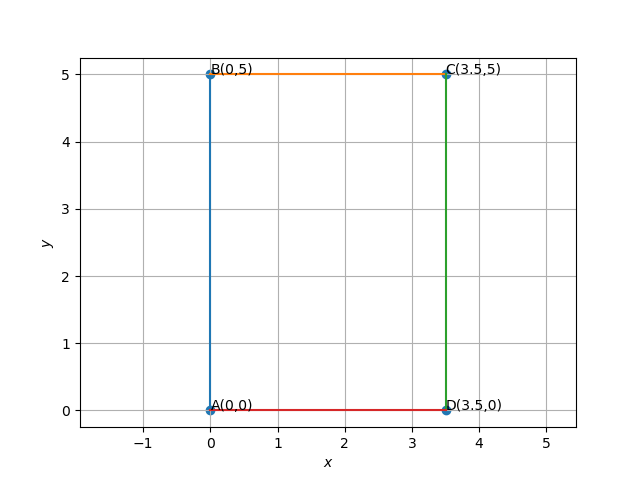
\includegraphics[width = 0.7\columnwidth]{../figs/img.png}
    \caption*{}
    \label{figs}
\end{figure}

\end{document}